\documentclass[12pt]{article}
\usepackage[a4paper]{geometry}
%\userpackage[top=1 in, bottom=1.25 in, left=1.1 in, rigth=1.1 in] {geometry}
%\usepackage[paperwidth=17cm, paperheight=22.5cm, bottom=2.5cm, right=2.5cm]{geometry}
\usepackage[utf8]{inputenc}
%\usepackage[a4paper, top=2.5cm, bottom=2.5cm, left=2.2cm, right=2.2cm]
%{geometry}
%\usepackage[myheadings]{fullpage}
\usepackage{fancyhdr}
\usepackage{lastpage}
%\usepackage{float}
\usepackage{graphicx, wrapfig, subcaption, setspace, booktabs}
\usepackage{graphicx}
\usepackage[T1]{fontenc}
\usepackage[font=small, labelfont=bf]{caption}
%\usepackage{fourier}
\usepackage[protrusion=true, expansion=true]{microtype}
\usepackage[english]{babel}
\usepackage{sectsty}
\usepackage{url, lipsum}
\usepackage[T1]{fontenc}
\usepackage{icomma}
\usepackage{siunitx}
\usepackage{ragged2e}
\usepackage{amsmath}
\usepackage{comment}
\usepackage{enumerate}
%\usepackage{changepage}
\usepackage{anysize}




\newcommand{\HRule}[1]{\rule{\linewidth}{#1}}
\onehalfspacing
\setcounter{tocdepth}{5}
\setcounter{secnumdepth}{5}

%-------------------------------------------------------------------------------
% HEADER & FOOTER
%-------------------------------------------------------------------------------


\begin{comment}
-Udledninger
$$
\begin{aligned}


\end{aligned}
$$

-Opgavetekst
\begin{figure}[H]
\includegraphics[width=0.5\textwidth]{"path"}
\end{figure} 


-Opgave billede med tekst
\begin{figure}[H]
\caption{"Billedtekst"}
\includegraphics[width=0.5\textwidth]{"path"}
\end{figure} 

-Værdier
$\\

$


\end{comment}
\begin{document}

\begin{titlepage}

\title{ \normalsize 
		%\begin{figure}
        \begin{center}
        
\includegraphics[height=6cm]{Logo.jpg}
        \end{center}
       % \end{figure}
        \LARGE \textsc{\textbf{Universidad De Sonora}} \\ \bigskip
		\Large División de Ciencias Exactas y Naturales \\
        Licenciatura En Física \\ \bigskip
        \bigskip
        Física Computacional I
		\\ [0.1cm]  
		\HRule{2pt} \\
		\Large \textbf{{Reporte de Actividad 1}} \\
        \textit{\textbf{"Atmósfera Terrestre"}}
		\HRule{2pt} \\
		\normalsize \vspace*{0.001\baselineskip}}
        
\date{\bigskip \Large Hermosillo, Sonora  \hspace*{\fill}  Enero 30 de 2018}

        
\author{
		\Large\textbf{ César Omar Ramírez Álvarez} \\ \bigskip
        \\ \bigskip
       \Large Profr. Carlos Lizárraga Celaya}
       \end{titlepage}
       \maketitle
       

\newpage
\pagestyle{plain}
\section{Introducción}
La atmósfera de la Tierra es la capa de gases, comúnmente conocida como aire, que rodea al planeta Tierra y es retenida por la gravedad de la Tierra. La atmósfera protege la vida en la Tierra al crear presión permitiendo que exista agua líquida en la superficie de la Tierra, absorbiendo radiación solar uv, calentando la superficie mediante retención de calor (efecto invernadero) y reduciendo las temperaturas extremas entre el día y la noche.

\begin{wrapfigure}{r}{0.36\textwidth} 
    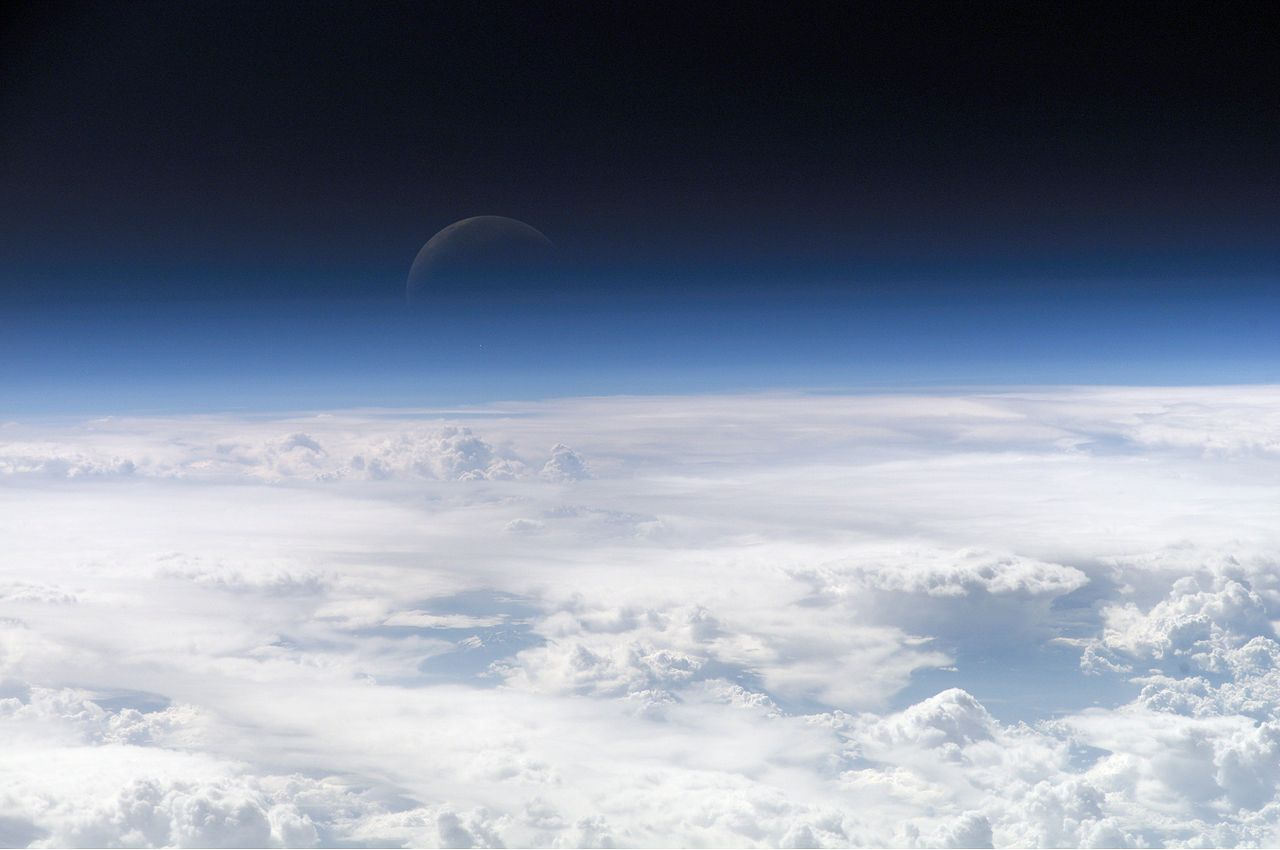
\includegraphics[width=0.36\textwidth]{Atmosfera.jpg}
    \caption{\textit{El color azúl mas visible que otras longitudes de onda.}}
\end{wrapfigure}

Por volumen, el aire seco contiene 78.09\% de nitrógeno, 20.95\% de oxígeno, 0.93\% de argón, 0.04\% de dióxido de carbono y pequeñas cantidades de otros gases. También contiene una cantidad variable de vapor de agua, en promedio alrededor de 1\% a nivel del mar, y 0.4\% en toda la atmósfera. El contenido de aire y la presión atmosférica varían en las diferentes capas, y el aire adecuado para su uso en la fotosíntesis por plantas y la respiración de animales terrestres se encuentra solo en la tropósfera y en atmósferas artificiales .

La atmósfera se vuelve más delgada y delgada a medida que aumenta la altitud, sin un límite definido entre la atmósfera y el espacio exterior .
\section{Composición}
	Los tres componentes principales del aire, y por lo tanto de la atmósfera de la Tierra, son nitrógeno, oxígeno y argón. El vapor de agua representa aproximadamente el 0.25\% de la atmósfera en masa. Los gases restantes a menudo se denominan gases traza, entre los cuales se encuentran los gases de efecto invernadero; principalmente dióxido de carbono, metano, óxido nitroso y ozono. El aire filtrado incluye trazas de muchos otros compuestos químicos.
    
\begin{wrapfigure}{l}{0.35\textwidth} 
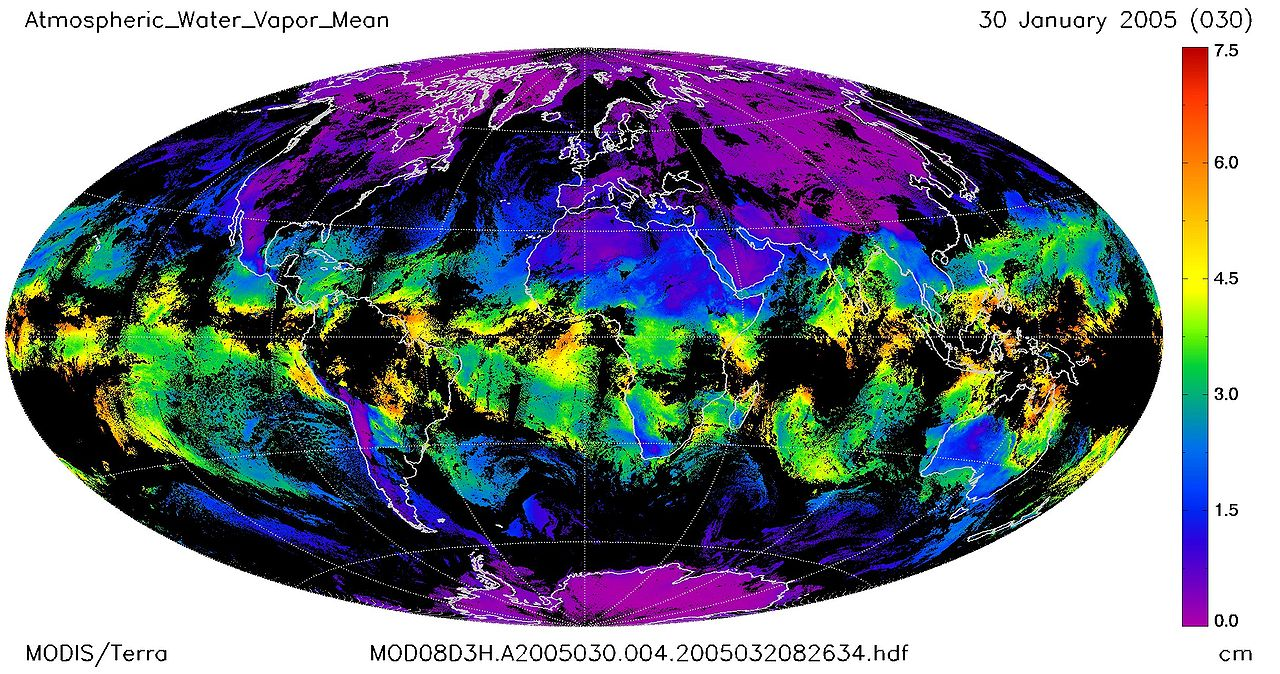
\includegraphics[width=0.35\textwidth]{Vapor.jpg}
\caption{\textit{Medida de vapor de agua atmósferico.}}
\end{wrapfigure}
    
    Muchas sustancias de origen natural pueden estar presentes en pequeñas cantidades,variables como aerosoles en una muestra de aire sin filtrar que incluye polvo de minerales y composición orgánica, polen y esporas, rocío de mar y cenizas volcánicas. Otros contaminantes industriales también pueden estar presentes en forma de gases o aerosoles, como cloro, compuestos de flúor y mercurio, compuestos de azufre que se pueden derivar de fuentes naturales o de la contaminación del aire industrial.\\
    
    
    
\section{Estructura De La Atmósfera}

\subsection{Capas Principales}
	En general, la presión del aire y la densidad disminuyen con la altitud en la atmósfera. Sin embargo, la temperatura tiene un perfil más complicado con la altitud, y puede permanecer relativamente constante o incluso aumentar con la altitud en algunas regiones. 
   
\begin{wrapfigure}{r}{0.4\textwidth} 
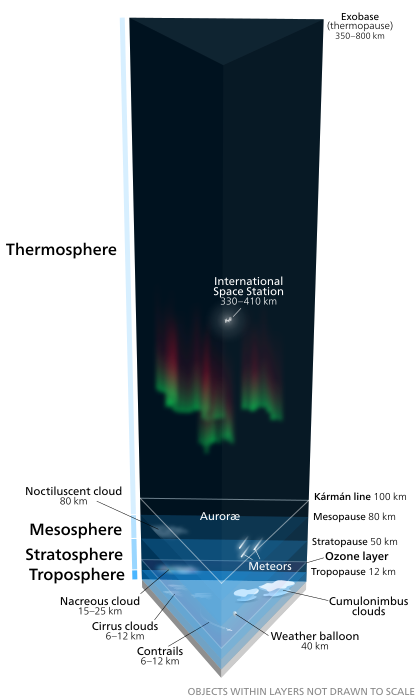
\includegraphics[width=0.4\textwidth]{Capas.png}
\caption{\textit{Atmósfera de la Tierra.}}
\end{wrapfigure}
   
    Debido a que el patrón general del perfil de temperatura / altitud es constante y medible por medio de sondeos de globo instrumentados, el comportamiento de la temperatura proporciona una medida útil para distinguir las capas atmosféricas. De esta manera, la atmósfera de la Tierra se puede dividir en cinco capas principales. \\
A continuación se explicarán de mayor a menor las cinco capas principales.

\subsubsection{Exósfera}
\textit{700 a 10,000 km (440 a 6,200 millas)}\\
La exósfera es la capa más externa de la atmósfera de la Tierra (es decir, el límite superior de la atmósfera). Esta capa está compuesta principalmente de densidades extremadamente bajas de hidrógeno, helio y varias moléculas más pesadas, incluyendo nitrógeno, oxígeno y dióxido de carbono más cerca de la exobase. Los átomos y las moléculas están tan separados que pueden viajar cientos de kilómetros sin colisionar entre sí. Por lo tanto, la exosfera ya no se comporta como un gas y las partículas escapan constantemente al espacio.

\subsubsection{Termósfera}
\textit{80 a 700 km (50 a 440 millas)}\\
La termósfera es la segunda capa más alta de la atmósfera de la Tierra. La temperatura de la termósfera aumenta gradualmente con la altura. La temperatura de esta capa puede elevarse hasta 1500 $^{\circ}$ C (2700 $^{\circ}$ F), aunque las moléculas de gas están tan separadas que su temperatura en el sentido habitual no es muy significativa.
Esta capa está completamente despejada y libre de vapor de agua.

\subsubsection{Mesósfera}
\textit{50 a 80 km (31 a 50 millas)}\\
La mesósfera es la tercera capa más alta de la atmósfera de la Tierra, ocupando la región sobre la estratosfera y debajo de la termosfera. Es el lugar más frío de la Tierra y tiene una temperatura promedio de alrededor de -85  $^{\circ}$ C (-120  $^{\circ}$ F ; 190  K ). 

\begin{wrapfigure}{r}{0.45\textwidth} 
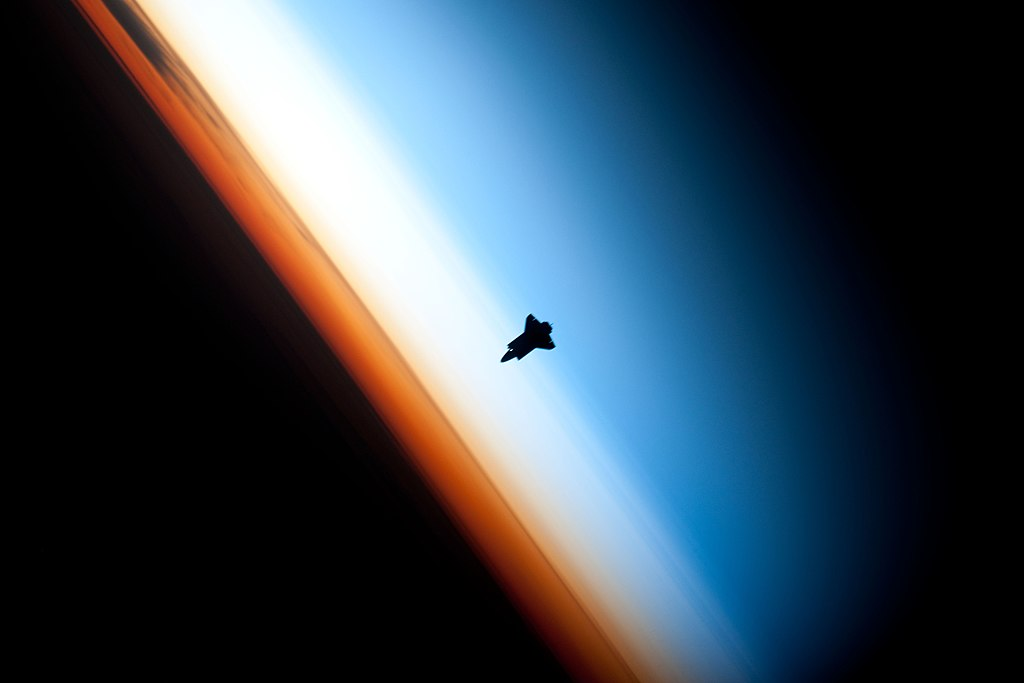
\includegraphics[width=0.45\textwidth]{explo.jpg}
\caption{\textit{Orbitando en la termósfera.}}
\end{wrapfigure}

Como dato se tiene que, está demasiado elevada sobre la Tierra para que sea accesible para aviones y globos propulsados por aviones a reacción, y demasiado bajo para permitir naves espaciales orbitales. La mesósfera se accede principalmente por cohetes que suenan y aviones propulsados por cohetes.

\subsubsection{Estratósfera}
\textit{12 a 50 km (7 a 31 millas)}\\
La estratósfera es la segunda capa más baja de la atmósfera de la Tierra. La presión atmosférica en la parte superior de la estratosfera es aproximadamente 1/1000 de la presión al nivel del mar. Contiene la capa de ozono, que es la parte de la atmósfera de la Tierra que contiene concentraciones relativamente altas de ese gas. La estratosfera define una capa en la que las temperaturas aumentan con el aumento de la altitud. Este aumento de la temperatura es causado por la absorción de la radiación de la radiación ultravioleta (UV) del Sol por la capa de ozono , que restringe la turbulencia y la mezcla. Aunque la temperatura puede ser de -60 $^{\circ}$ C (-76 $^{\circ}$ F, 210 K) en la tropopausa, la parte superior de la estratoófera está mucho más caliente y puede estar cerca de 0 $^{\circ}$ C.

\subsubsection{Tropósfera}
\textit{0 a 12 km (de 0 a 7 millas)}\\
La tropósfera es la capa más baja de la atmósfera de la Tierra. Aunque se producen variaciones, la temperatura generalmente disminuye con el aumento de la altitud en la tropósfera porque la tropósfera se calienta principalmente a través de la transferencia de energía desde la superficie. Por lo tanto, la parte más baja de la tropósfera (es decir, la superficie de la Tierra) suele ser la sección más cálida de la tropósfera. Contiene aproximadamente el 80\% de la masa de la atmósfera de la Tierra. La troposfera es más densa que todas las capas atmosféricas que la recubren porque un peso atmosférico más grande se encuentra en su parte superior y hace que se comprima más severamente.

El 50\%de la masa total de la atmósfera se encuentra en los 5,6 km más bajos de la tropósfera.
Casi todo el vapor de agua atmosférico o humedad se encuentra en la tropósfera, por lo que es la capa donde tiene lugar la mayor parte del clima de la Tierra.
\subsection{Otras Capas}
Dentro de las cinco capas principales que están determinadas en gran medida por la temperatura, varias capas secundarias se pueden distinguir por otras propiedades:\\
\begin{itemize}
\item La \textit{capa de ozono} está contenida dentro de la estratósfera. En esta capa, las concentraciones de ozono son aproximadamente de 2 a 8 ppm. Se encuentra en la porción inferior de la estratósfera desde aproximadamente 15-35 km (9.3-21.7 millas), aunque el espesor varía estacional y geográfica. \\
\item La \textit{ionósfera} es una región de la atmósfera ionizada por la radiación solar. Durante el día, se extiende de 50 a 1,000 km (31 a 621 millas) e incluye la mesósfera, la termósfera y partes de la exósfera.\\
\item La \textit{homósfera} y la \textit{heterósfera} se definen según si los gases atmosféricos están bien mezclados.\\
\item La \textit{capa límite planetaria} es la parte de la tropósfera más cercana a la superficie de la Tierra y directamente afectada por ella, principalmente a través de la difusión turbulenta. Durante el día, la capa límite planetaria suele estar bien mezclada, mientras que por la noche se estratifica de manera estable con una mezcla débil o intermitente.
\end{itemize}


\section{Propiedades Físicas}

\subsection{Presión Y Espesor}
La presión atmosférica promedio a nivel del mar está definida por la Atmósfera Estándar Internacional como 101325 pascales. Que a su vez se conoce como una unidad estándar, la atmósfera (atm). La masa atmosférica total es $5.1480 \times 10 ^{18}$ kg ($1.135 \times10 ^{19}$ lb), aproximadamente un 2.5\% menos de lo que se deduciría de la presión media del nivel del mar y el área de la Tierra de 51007,2 megahectáreas, esta parte está desplazada por el terreno montañoso de la Tierra. Aclarando que también la presión del aire varía, según ubicación y el clima debido a que la presión atmósferica es peso del aire entre unidad de aire donde se mide. La masa disminuye exponencialmente con la altitud, cayendo a la mitad cada 5,6 km  o por un factor de $\frac{1}{e}$ cada 7,64 km. 

De manera general, podriamos decir que la masa de la atmósfera se distribuye de la siguiente manera:\\
$\to$ 50\% está por debajo de 5.6 km.\\
$\to$ 90\% está por debajo de 16 km.\\
$\to$ 99.99997\% está por debajo de 100 km, \textit{la línea Kármán} (Astronautas).


\subsection{Temperatura Y Velocidad Del Sonido}
La temperatura disminuye con la altitud comenzando al nivel del mar, pero las variaciones comienzan por encima de los 11 km. En la estratósfera, comenzando por encima de unos 20 km, la temperatura aumenta con la altura, debido al calentamiento dentro de la capa de ozono causado por la captura de radiación uv del Sol por el dioxígeno y el gas ozono en esta región. Otra región de aumento de la temperatura con la altitud se produce a altitudes muy altas, en la termósfera  nombrada por encima de 90 km.

Debido a que en un gas ideal de composición constante, la velocidad del sonido depende únicamente de la temperatura y no de la presión o densidad del gas, la velocidad del sonido en la atmósfera con la altitud adquiere la forma del perfil de temperatura complicado y no refleja los cambios altitudinales en densidad o presión.

\subsection{Densidad Y Masa}
La densidad del aire a nivel del mar es de aproximadamente 1.2 kg/m$^3$. La densidad se calcula a partir de mediciones de temperatura, presión y humedad utilizando la ecuación de estado para el aire.\\
\begin{wrapfigure}{r}{0.45\textwidth} 
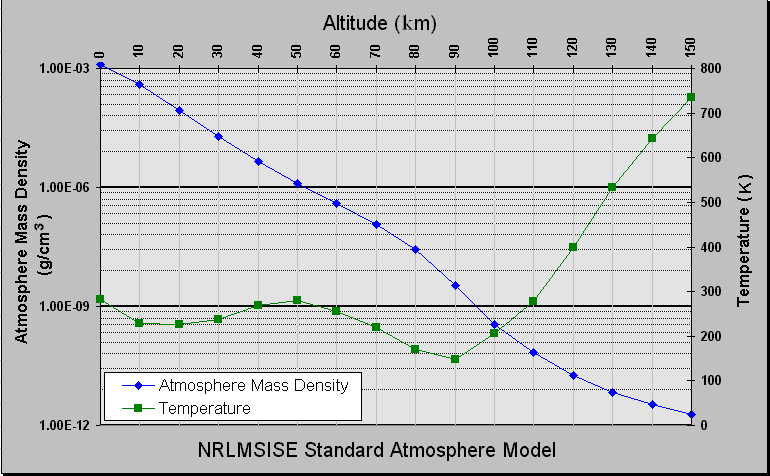
\includegraphics[width=0.45\textwidth]{model.png}
\caption{\textit{Temperatura y densidad de masa frente a la altitud del modelo de atmósfera estándar.}}
\end{wrapfigure}La densidad atmosférica disminuye a medida que aumenta la altitud. Esta variación se puede modelar aproximadamente utilizando la fórmula barométrica.

La masa promedio de la atmósfera es de aproximadamente 5$\times 10 ^{15}$ toneladas. Mientras que el Centro Nacional Americano de Investigación Atmosférica consideran otra cifra, ya que toman en cuenta un rango anual debido al vapor de agua.

\section{Propiedades Ópticas}
La radiación solar es la energía que recibe la Tierra del Sol. La Tierra también emite radiación hacia el espacio, pero a longitudes de onda más largas que no podemos ver. Parte de la radiación entrante y emitida es absorbida o reflejada por la atmósfera. 

\subsection{Dispersión}
Cuando la luz pasa a través de la atmósfera de la Tierra, los fotones interactúan con ella a través de la dispersión . Si la luz no interactúa con la atmósfera, se llama \textit{radiación directa}. La \textit{radiación indirecta} es luz que se ha dispersado en la atmósfera.

\subsection{Absorción}
Diferentes moléculas absorben diferentes longitudes de onda de radiación. Cuando una molécula absorbe un fotón, aumenta la energía de la molécula. Esto calienta la atmósfera, pero la atmósfera también se enfría al emitir radiación.

Los espectros de absorción combinados de los gases en la atmósfera dejan "ventanas" de baja opacidad , permitiendo la transmisión de solo ciertas bandas de luz. La ventana óptica se extiende desde alrededor de 300 nm hasta el rango que los humanos pueden ver, el espectro visible, a aproximadamente 400-700 nm y continúa al infrarrojo a alrededor de 1100 nm. También hay ventanas de infrarrojos y de radio que transmiten algunas ondas infrarrojas y de radio a longitudes de onda más largas.

\subsection{Emisión}
La emisión es cuando un objeto emite radiación. Los objetos tienden a emitir cantidades y longitudes de onda de radiación dependiendo de sus curvas de emisión de "cuerpo negro", por lo tanto, los objetos más calientes tienden a emitir más radiación, con longitudes de onda más cortas. Los objetos más fríos emiten menos radiación, con longitudes de onda más largas.

 La Tierra tiene aproximadamente 290 K, por lo que su radiación alcanza un máximo cercano a las 10,000 nm, y es demasiado larga para ser visible para los humanos. Debido a su temperatura, la atmósfera emite radiación infrarroja. El efecto invernadero está directamente relacionado con este efecto de absorción y emisión.
 
\subsection{Índice De Refracción}
El índice de refracción del aire es cercano, pero apenas superior a 1. Las variaciones sistemáticas en el índice de refracción pueden conducir a la flexión de los rayos de luz en recorridos ópticos largos. Éste índice depende de la temperatura, dando lugar a efectos de refracción cuando el gradiente de temperatura es grande.\\
\begin{wrapfigure}{r}{0.45\textwidth} 
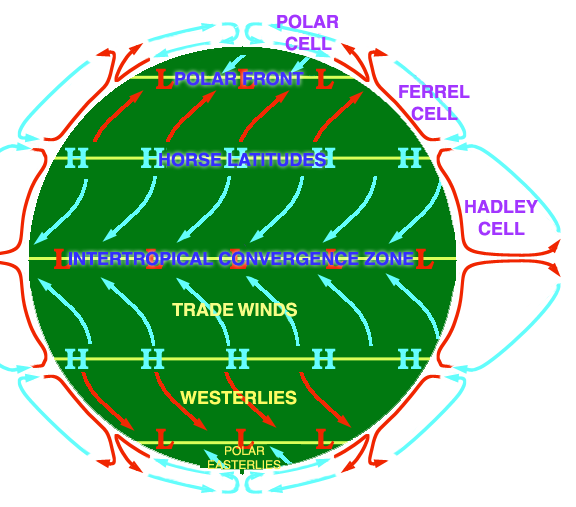
\includegraphics[width=0.45\textwidth]{circ.png}
\caption{\textit{Tres celdas de gran circulación.}}
\end{wrapfigure}
\subsection{Circulación}
La circulación atmosférica es el movimiento de aire a gran escala a través de la troposfera, y los medios por los cuales se distribuye el calor alrededor de la Tierra. La estructura a gran escala de la circulación atmosférica varía de un año a otro, pero la estructura básica permanece bastante constante porque está determinada por la velocidad de rotación de la Tierra y la diferencia en la radiación solar entre el ecuador y los polos.

\section{Bibliografía}
\begin{itemize}
\item Atmosphere of Earth. (2018,29 de Enero). Obtenido de 						 https://en.wikipedia.org/wiki/Atmosphere\_of\_Earth
\end{itemize}

\section{Apéndice}
\begin{enumerate}
\item \textbf{¿Qué fue lo que más te llamó la atención de esta actividad?}\\
\textit{Primeramente, familiarizarme con LATEX ya que esta actividad me llevó a hacer uso de él para lo cual, siento que aunque es la primera (de muchas) ya conozco algo básico. Por otro lado, el realizar esta actividad me introdujo al ambiente de trabajo que usaremos durante el curso de Física Computacional y a su vez conocí datos muy importantes sobre nuestra atmósfera terrestre.}
\item \textbf{¿Qué fue lo que se te hizo menos interesante?}\\
\textit{En principio, el echo de que no pudiera manipular muy rapidamente la estética del documento ya que me gusta arreglar ciertas cosas (imágenes) a mi modo, pero despúes trate de mejorar en ese aspecto. Por otro lado, que sea una página en línea a veces (en su mayoría) se pone lenta. }
\item \textbf{¿Qué cambios harías para mejorar esta actividad?} \\
\textit{Sinceramente nada, ya que todo está muy completo y es muy buena introducción para el uso de LATEX.}
\item \textbf{¿Cuál es tu primera impresión de uso de LATEX?}\\
Muy padre, antes le tenía miedo, ahora me gusta explorar todas sus variedades que tiene, y vaya que sí, resalto quer nunca lo habia usado y tardé alrededor de 3 horas para hacer la portada.
\item \textbf{¿El tiempo sugerido para esta actividad fue suficiente? }\\
Fue justo y necesario. Aunque me atrasé por hacer otras actividades.
\item \textbf{¿Encontraste algún documento o recurso en línea útil que quisieras compartir con los demás? } \\
\textit{Leí varios a lo largo de estos días de la actividad, pero comentando con mis compañeros, todos coincidiamos en las cosas en las que buscamos para salir de dudas, lamentablemente no los compartí pero un compañero si compartió un pdf muy importante.}

\end{enumerate}

\end{document}